\documentclass[11pt,fleqn]{article}

\textheight=23.3cm
\textwidth=16.5cm
\topmargin=-15mm
\oddsidemargin=0cm

\usepackage{enumerate}
\usepackage{amsmath}
\usepackage{amssymb}
\usepackage{bbm}
\usepackage{ulem}
\usepackage{graphicx}
\usepackage{wrapfig}
\usepackage{pdflscape}
\usepackage[sidewaysfigure]{rotating}
\usepackage{natbib}
\usepackage{multirow}
\newcommand{\tb}{\hspace*{3mm}}
\bibpunct{(}{)}{;}{a}{,}{,}
\parskip=3mm
\parindent=5mm
\baselineskip=17pt

\usepackage{amsthm}
\newtheorem{assumption}{Assumption}
\newtheorem{definition}{Definition}
\newtheorem{proposition}{Proposition}
\newtheorem{corollary}{Corollary}
\newtheorem{lemma}{Lemma}
\newtheorem{theorem}{Theorem}
\renewcommand{\qedsymbol}{\textit{Q.E.D.}}

\DeclareMathOperator*{\argmax}{arg\,max}
\DeclareMathOperator*{\argmin}{arg\,min}

\usepackage{hyperref}
\hypersetup{
  pdftitle={Replication of Huggett, Ventura \& Yaron (2006) - Human Capital and Earnings Distribution Dynamics},
  pdfauthor={Robert Kirkby},
  colorlinks=true,
  linkcolor=black,
  citecolor=black,
  urlcolor=blue,
  breaklinks=true
}


\begin{document}


%===============================
\newcommand{\rob}[1]{{\noindent\color{blue}\bf #1}}
\newcommand{\robc}[1]{{\noindent\color{blue}\bf R: #1}}
%===============================

\title{Replication of Huggett, Ventura \& Yaron (2006) - Human Capital and Earnings Distribution Dynamics}
\author{Robert Kirkby}
\date{\today}
\maketitle

Brief description of a replication of \cite*{HuggettVenturaYaron2006}, hereafter HVY2006. This is not intended as a full description of the model; rather, the goal is to show how the model is expressed in terms of the VFI Toolkit. For a full description see the original paper.

The replication covers all of the tables (1--6) and figures (1--6) of the paper, both the empirical part (the age profiles of the earnings distribution in the PSID) and the model part, for all five values of the curvature parameter $\alpha$ and both starting ages (10 and 20), and for both the parametric and the non-parametric initial distribution. It also reproduces the cross-section comparison at the end of Section 5.1, and checks Proposition 1(iii) numerically. Everything is run by \verb|HuggettVenturaYaron2006.m| including the data work and the model.

Everything replicates, with only minor quantitative differences. The replication is in some sense substantial overkill. The parameters to be calibrated do not appear in the value function problem; they only matter for the agent distribution. HVY2006 exploit this: for each value of $\alpha$ and starting age they solve the value function once, and then calibrate by iterating only on the agent distribution and model statistics. Since the value function is by far the most computationally costly part of the model, this massively reduces the difficulty of the problem. By contrast, the replication just uses the VFI Toolkit calibration commands, and so solves the value function at every iteration.

The rest of this document was largely written by Claude.

\section{Model description}

The model is a Ben-Porath human capital model. An agent works from model period $j=1$ to $J$, which is either age 20 to 58 ($J=39$) or age 10 to 58 ($J=49$). The state is human capital, $h$, and learning ability, $a$, which is fixed over the life cycle. Each period the agent splits their time between market work and producing new human capital, choosing the fraction of time $l\in[0,1]$ spent producing human capital. Earnings are $w_j h (1-l)$, where the rental rate of human capital grows deterministically, $w_j=(1+g)^{j-1}$, and human capital evolves as
\begin{align*}
 h' = a (h l)^\alpha + (1-\delta) h.
\end{align*}
Agents maximize the present value of earnings,
\begin{align*}
 V_j(h,a) = & \max_{l\in[0,1]} \; w_j h (1-l) \; + \; \frac{1}{1+r}\, V_{j+1}(h',a) \\
 \text{subject to } & h' = a (h l)^\alpha + (1-\delta) h, \qquad V_{J+1}=0.
\end{align*}
Agents differ only in their initial human capital and learning ability, $(h_1,a)$, and the joint distribution of these at the initial age is chosen so that the model best reproduces the age profiles of mean earnings, earnings dispersion (the Gini coefficient) and earnings skewness (mean/median) in the PSID. Parameter values are in Table \ref{tab:HVY2006_Table1}.

\subsection{Closed-form solution}

HVY2006 Proposition 1(ii) gives a closed-form solution. The value function is linear in $h$, with slope $\lambda_j=w_j+\frac{1-\delta}{1+r}\lambda_{j+1}$ ($\lambda_{J+1}=0$), and the human capital put into producing new human capital is
\begin{align*}
 x_j \equiv h\,l = \min\!\left\{ h,\; \left(\frac{\lambda_{j+1}\,\alpha\, a}{(1+r)\,w_j}\right)^{1/(1-\alpha)} \right\},
\end{align*}
so that an agent spends all their time producing human capital ($l=1$) while $h$ is below an age and ability dependent cutoff. The VFI Toolkit solves the model numerically (below), and the closed form is used where the numerical solution's discretization of $l$ matters: the persistence of earnings growth rates (Table 6) is very sensitive to $l$ moving in steps of $0.01$ on the grid. The closed form reproduces the toolkit's mean earnings profile to within 0.3\% at every age.


\section{VFI Toolkit implementation}

\begin{itemize}
 \item Human capital is an \emph{experience asset}: next period's $h'$ is a deterministic function of this period's decision $l$ and of $h$, set by \verb|vfoptions.experienceasset=1| and \verb|vfoptions.aprimeFn|. The grid on $h$ is 501 points on $[0.1,1000]$, and the grid on $l$ is 101 points on $[0,1]$. The return function is earnings, $w_j h (1-l)$, and the discount factor is $1/(1+r)$.
 \item Learning ability is a \emph{permanent type}: 21 ability levels on a grid for $\log(a)$ (discretized as normal using \cite{FarmerToda2017}). The grid itself depends on the mean and standard deviation of $\log(a)$, which are calibrated, so it is rebuilt at each step of the calibration using a \verb|PTypeParamFn|.
 \item The initial distribution is given as a function (\verb|jequaloneDistFn|): a bivariate log-normal on $(h_1,a)$, evaluated on the grids for $h$ and ability. The correlation is parametrized as in Archakov \& Hansen (2021), which for a $2\times2$ correlation matrix means the correlation of the logs is $\tanh(\gamma)$ for an unrestricted parameter $\gamma$ (restricted to $[-3,3]$, so the correlation lies in $(-0.995,0.995)$).
 \item The parametric case calibrates the five parameters of the log-normal (two means, two standard deviations, and the correlation) using \verb|CalibrateLifeCycleModel_PType|, minimizing the sum over ages 20--58 of the squared log ratio of data to model for mean earnings, the Gini coefficient, and mean/median (HVY2006 footnote 18). There are ten cases: $\alpha=0.5,0.6,0.7,0.8,0.9$ and starting ages 10 and 20. The initial guess for each case is the log-normal implied by the paper's Table 5 values for that case. The calibrated parameters are in Table \ref{tab:HVY2006_CalibParams}.
\end{itemize}

\subsection{The non-parametric case}

In the non-parametric case the initial distribution is any histogram on a rectangular grid of 20 points for initial human capital and 20 points for ability (400 bins). The model solution does not depend on the initial distribution, and given the closed-form solution each bin $(h_1,a)$ gives one deterministic earnings path, so the earnings distribution at each age is the 400 paths weighted by the histogram. We therefore calibrate the 400 weights directly, parametrized as $\exp(\theta)/\sum\exp(\theta)$, with the same objective as the parametric case, using \verb|lsqnonlin| (Levenberg--Marquardt, as there are more weights than targets). The grids span $\pm2.5$ standard deviations of $\log(h_1)$ and $\log(a)$ from the parametric calibration of the same case, and the parametric calibration is the initial guess.

\subsection{Fixed initial human capital (Fig 6)}

For Fig 6, everyone starts (at age 10, $\alpha=0.7$) with the same initial human capital, and only ability differs, as a histogram on 20 ability levels (HVY2006 footnote 21). The ability weights are calibrated as in the non-parametric case for a given common $h_1$, and the common $h_1$ is chosen by a grid search over 81 values.


\section{Data}

The data are the PSID family files 1969--1992, male household heads aged 18--60 (for the 5-year age bins centred on ages 20 to 58), with strictly positive earnings (head's labor income), excluding the SEO subsample. The broad sample includes those working, temporarily laid off, unemployed, or students; note that the PSID changes the coding of employment status in 1976. Labor income in the year $t$ family file is for calendar year $t-1$, and is deflated by the CPI for that year.

For each age $j$ and year $t$ we compute 23 earnings percentiles $e^p_{j,t}$ (using a 5-year age bin), and regress the log percentiles on age and cohort dummies (HVY2006 equation 2). The age effects are scaled to pass through the geometric average of $e^p_{40,t}$ across years, and so that mean earnings at age 58 equal 100 (Figs 1 and 2). Mean earnings, the Gini coefficient and mean/median are computed from the 23 percentiles, each percentile standing for a mass of the population. Fig 3 shows the two alternative views of the age effects: time dummies instead of cohort dummies, and cohort dummies plus time effects restricted to be mean zero and orthogonal to a time trend.


\section{Results}

The age profiles of the earnings distribution in the PSID (Figs 1--3) are close to HVY2006 for dispersion and skewness. Mean earnings rise less steeply in our data: mean earnings at age 20 are about 43 (with age 58 equal to 100), against about 55 in HVY2006. This is not explained by the choice of sample (narrow sample, excluding students, or the timing of the CPI each move it by at most 3), and the most likely explanations are the exact earnings variable or later revisions of the PSID files. It is the reason the calibrated mean initial human capital is about 10 lower than in HVY2006 throughout Tables 4 and 5. The average number of observations per panel-year is 2108, against 2137 in HVY2006.

The model results replicate well:
\begin{itemize}
 \item Goodness of fit (Table \ref{tab:HVY2006_Table2}): as in HVY2006, the non-parametric case fits much better than the parametric case, and the fit is similar to HVY2006's (a little better, except for $\alpha=0.9$).
 \item Initial distributions (Tables \ref{tab:HVY2006_Table4} and \ref{tab:HVY2006_Table5}): learning ability is very close to HVY2006 throughout. The correlation of ability and initial human capital is high when accumulation starts at age 20 and much lower when it starts at age 10, as in HVY2006.
 \item Variance decomposition (Table \ref{tab:HVY2006_Table3}): in the parametric case, learning ability accounts for 70--79\% of the variance of the present value of earnings, against 65--79\% in HVY2006. In the non-parametric case we find a larger role for ability than HVY2006. With 400 weights and 117 targets, the targets do not pin down the variance decomposition, so it depends on which of the many histograms that fit the data equally well the calibration lands on; the non-parametric row of Table 3 should be read with this in mind.
 \item Persistence (Table \ref{tab:HVY2006_Table6}): the correlations of earnings levels and growth rates are very close to HVY2006 (note HVY2006 report the non-parametric case, accumulation from age 10; ours is the parametric case).
 \item Cross-section (Table \ref{tab:HVY2006_CrossSection}): constructing the cross-section earnings distribution from the age profiles with 1\% population growth, as in HVY2006, both the data and the model are close to the HVY2006 values, which the model was not calibrated to.
 \item Fixed initial human capital (Fig \ref{fig:HVY2006_Fig6}): with a common initial human capital the model generates a pronounced U-shape in earnings dispersion (lowest at age 27; HVY2006 report about age 24) and fits the data much worse (mean absolute deviation of 12.3\%, against 2.0\% in the non-parametric case).
 \item Proposition 1(iii) (Table \ref{tab:HVY2006_GiniByAge} and Fig \ref{fig:HVY2006_Prop1}): if every agent has the same ability, the Lorenz curves of human capital and of earnings become more equal at every age, and the Gini coefficient of earnings falls from 0.34 to 0.16 over the life cycle; differences in learning ability are essential for rising dispersion.
\end{itemize}


\section{Deviations from the paper}

\begin{itemize}
 \item Grids: 21 ability levels (rather than 20) in the parametric case, and a fine grid on human capital (501 points). The time devoted to human capital is on a grid of 101 points in the toolkit solution; the closed-form solution is used for Table 6, the non-parametric case and Fig 6.
 \item Present value of earnings (Table 3): as of age 20 for both starting ages, as HVY2006 state; for accumulation from age 10, this is the value at age 20 weighted by the distribution of agents at age 20.
 \item Non-parametric grids: the $20\times20$ grids span $\pm2.5$ standard deviations of the parametric calibration; for $\alpha=0.9$ about 5--7\% of the mass lies on the edge of the grid. A wider grid ($\pm3$) was tried and did not improve the fit.
 \item Table 6 is reported for the parametric case (both starting ages); HVY2006 report the non-parametric case from age 10.
\end{itemize}


\bibliographystyle{plainnat}
\bibliography{/home/kmarshallbanana/Dropbox/RDKbiblio.bib}


%%%%%%%%%%%%%%%%%%%%%%%%%%%%%%%%%%%%%%%%%%%%%%%%%%%
\clearpage
\section*{Tables}

\begin{table}[htp]
\caption{Table 1 of HVY2006: parameter values. Top: original from paper. Bottom: replication.}
\label{tab:HVY2006_Table1}
\begin{center}
\begin{tabular}{c}
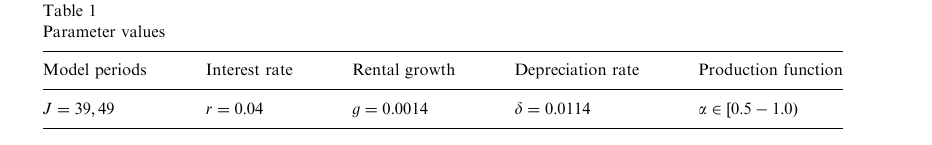
\includegraphics[width=140mm]{./OriginalTablesFigures/HVY2006_Table1.png}
\end{tabular}
\end{center}
\begin{center}
\input{../SavedOutput/LatexInputs/HVY2006_Table1.tex}
\end{center}
\end{table}

\begin{table}[htp]
\caption{Table 2 of HVY2006: mean absolute deviation (\%) between model and data. Top: original from paper. Bottom: replication.}
\label{tab:HVY2006_Table2}
\begin{center}
\begin{tabular}{c}
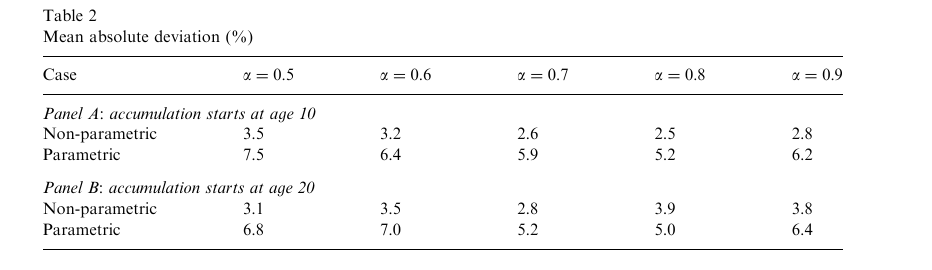
\includegraphics[width=140mm]{./OriginalTablesFigures/HVY2006_Table2.png}
\end{tabular}
\end{center}
\begin{center}
\input{../SavedOutput/LatexInputs/HVY2006_Table2.tex}
\end{center}
\end{table}

\begin{table}[htp]
\caption{Table 3 of HVY2006: percentage of the variance in the present value of earnings (as of age 20) due to learning ability differences. Top: original from paper. Bottom: replication.}
\label{tab:HVY2006_Table3}
\begin{center}
\begin{tabular}{c}
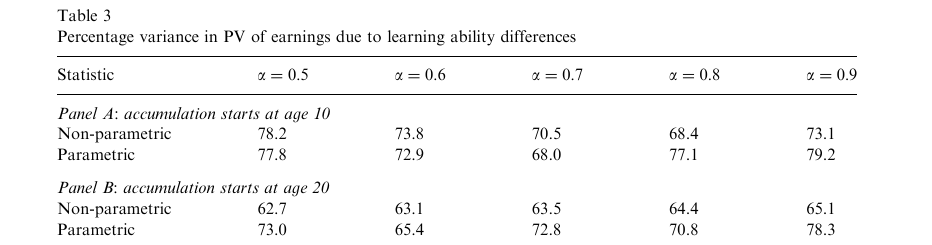
\includegraphics[width=140mm]{./OriginalTablesFigures/HVY2006_Table3.png}
\end{tabular}
\end{center}
\begin{center}
\input{../SavedOutput/LatexInputs/HVY2006_Table3.tex}
\end{center}
\end{table}

\begin{table}[htp]
\caption{Table 4 of HVY2006: ability and human capital at birth, non-parametric case. Top: original from paper. Bottom: replication.}
\label{tab:HVY2006_Table4}
\begin{center}
\begin{tabular}{c}
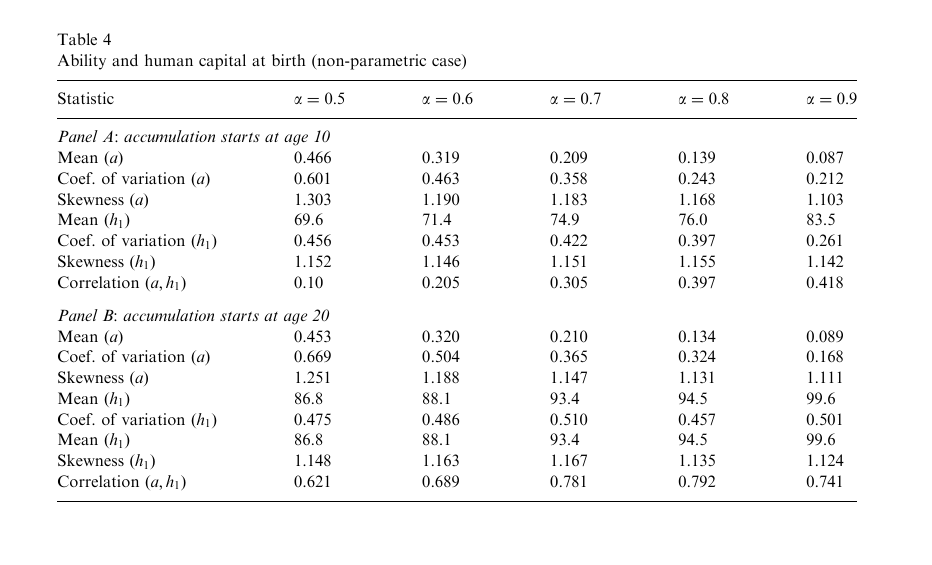
\includegraphics[width=130mm]{./OriginalTablesFigures/HVY2006_Table4.png}
\end{tabular}
\end{center}
\begin{center}
\footnotesize
\input{../SavedOutput/LatexInputs/HVY2006_Table4.tex}
\end{center}
\end{table}

\begin{table}[htp]
\caption{Table 5 of HVY2006: ability and human capital at birth, parametric case. Top: original from paper. Bottom: replication.}
\label{tab:HVY2006_Table5}
\begin{center}
\begin{tabular}{c}
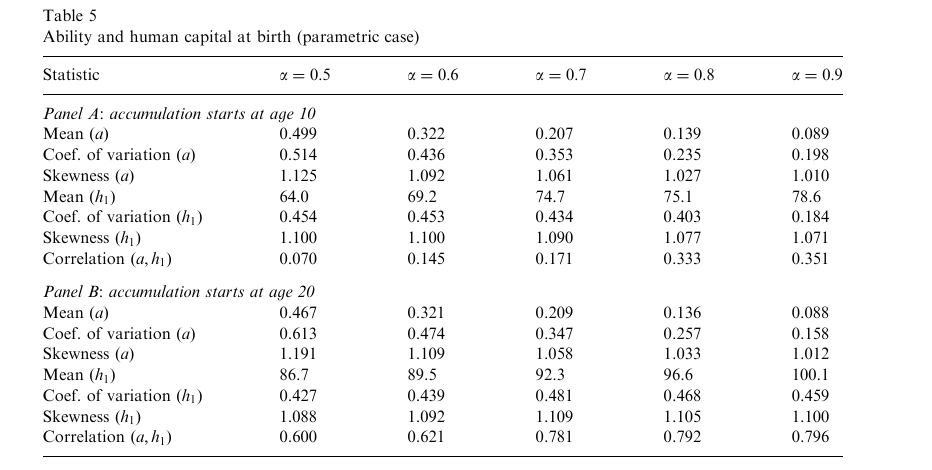
\includegraphics[width=130mm]{./OriginalTablesFigures/HVY2006_Table5.png}
\end{tabular}
\end{center}
\begin{center}
\footnotesize
\input{../SavedOutput/LatexInputs/HVY2006_Table5.tex}
\end{center}
\end{table}

\begin{table}[htp]
\caption{Table 6 of HVY2006: persistence in individual earnings, $\alpha=0.7$. Top: original from paper (non-parametric case, accumulation from age 10). Bottom: replication (parametric case). $E_j$ is earnings and $z_j=\log(E_j/E_{j-1})$ is earnings growth.}
\label{tab:HVY2006_Table6}
\begin{center}
\begin{tabular}{c}
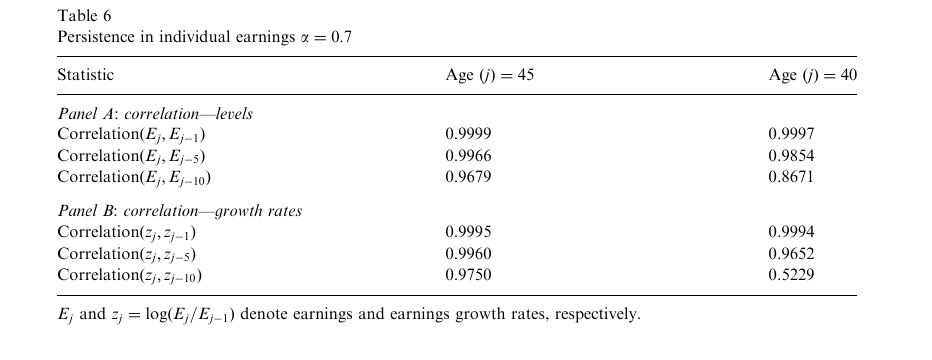
\includegraphics[width=140mm]{./OriginalTablesFigures/HVY2006_Table6.png}
\end{tabular}
\end{center}
\begin{center}
\input{../SavedOutput/LatexInputs/HVY2006_Table6.tex}
\end{center}
\end{table}

\begin{table}[htp]
\caption{Cross-section earnings distribution (HVY2006 Section 5.1), $\alpha=0.7$: ages 20--58 pooled with 1\% population growth. Top shares are the percentage of all earnings received by the top 20\%, 10\%, 5\% and 1\% of earners.}
\label{tab:HVY2006_CrossSection}
\begin{center}
\small
\input{../SavedOutput/LatexInputs/HVY2006_CrossSection.tex}
\end{center}
\end{table}

\begin{table}[htp]
\caption{Gini coefficient of earnings by age: data, the baseline model, the model where every agent has the mean ability (Proposition 1(iii)), and the model with a common initial human capital (Fig 6).}
\label{tab:HVY2006_GiniByAge}
\begin{center}
\small
\input{../SavedOutput/LatexInputs/HVY2006_GiniByAge.tex}
\end{center}
\end{table}

\begin{table}[htp]
\caption{Calibrated parameters, parametric case: the joint log-normal distribution of initial human capital and learning ability.}
\label{tab:HVY2006_CalibParams}
\begin{center}
\input{../SavedOutput/LatexInputs/HVY2006_CalibParams.tex}
\end{center}
\end{table}


%%%%%%%%%%%%%%%%%%%%%%%%%%%%%%%%%%%%%%%%%%%%%%%%%%%
\clearpage
\section*{Figures}

\begin{figure}[htp]
\begin{center}
\begin{tabular}{cc}
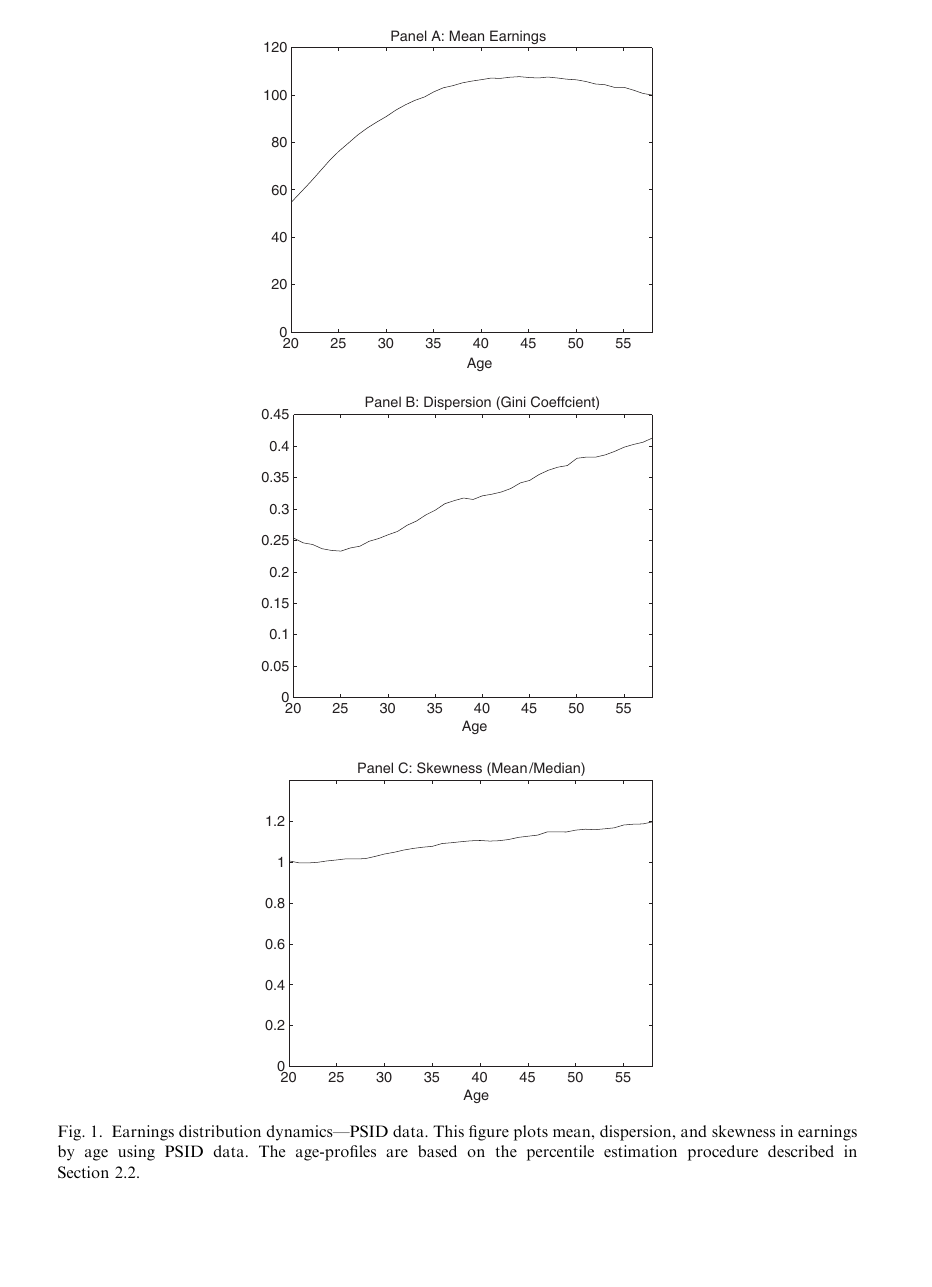
\includegraphics[height=18cm,trim=120.5 83.5 129.1 9.6,clip]{./OriginalTablesFigures/HVY2006_Figure1.png} & \includegraphics[height=18cm,trim=12.0 65.3 24.5 50.4,clip]{../SavedOutput/Graphs/HVY2006_Fig1.png}
\end{tabular}
\end{center}
\caption{Figure 1 of HVY2006: earnings distribution dynamics, PSID data. Left: original from paper. Right: replication.}
\label{fig:HVY2006_Fig1}
\end{figure}

\begin{figure}[htp]
\begin{center}
\begin{tabular}{c}
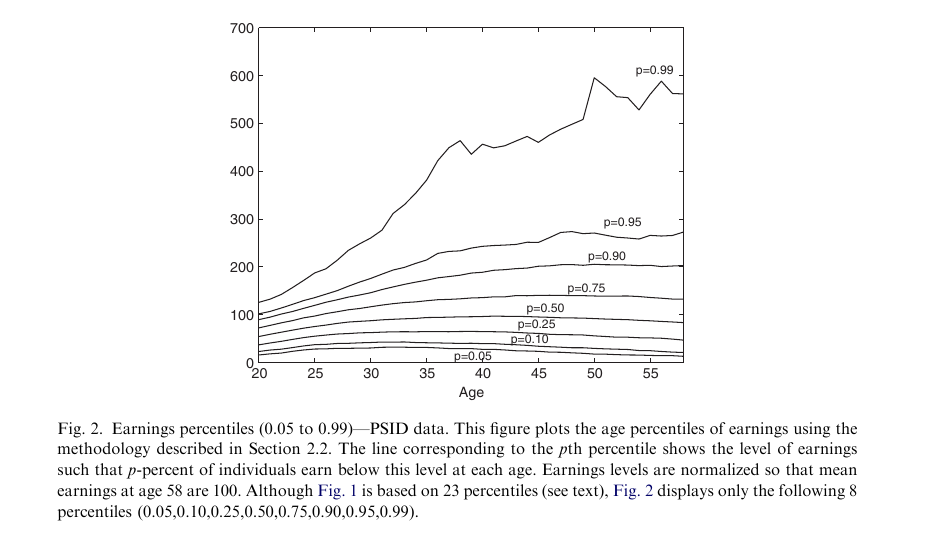
\includegraphics[width=110mm]{./OriginalTablesFigures/HVY2006_Figure2.png} \\
\includegraphics[width=110mm]{../SavedOutput/Graphs/HVY2006_Fig2.png}
\end{tabular}
\end{center}
\caption{Figure 2 of HVY2006: earnings percentiles (0.05 to 0.99), PSID data. Top: original from paper. Bottom: replication.}
\label{fig:HVY2006_Fig2}
\end{figure}

\begin{figure}[htp]
\begin{center}
\begin{tabular}{cc}
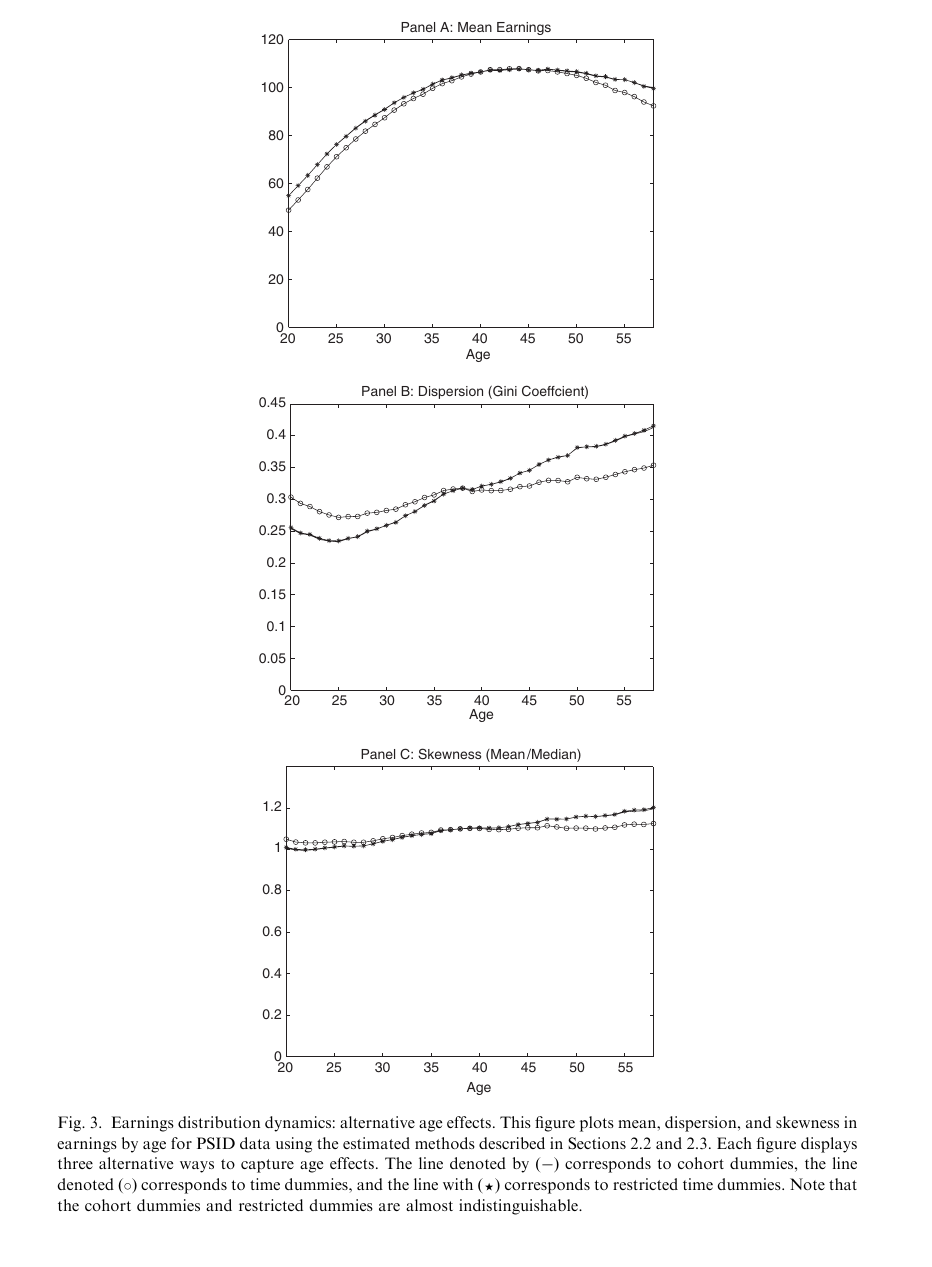
\includegraphics[height=18cm,trim=119.5 77.8 127.2 5.8,clip]{./OriginalTablesFigures/HVY2006_Figure3.png} & \includegraphics[height=18cm,trim=12.0 65.3 24.5 50.4,clip]{../SavedOutput/Graphs/HVY2006_Fig3.png}
\end{tabular}
\end{center}
\caption{Figure 3 of HVY2006: alternative views of the age effects (cohort dummies, time dummies, restricted time dummies). Left: original from paper, where the line ($-$) is cohort dummies, ($\circ$) time dummies and ($\star$) restricted time dummies. Right: replication.}
\label{fig:HVY2006_Fig3}
\end{figure}

\begin{figure}[htp]
\begin{center}
\begin{tabular}{cc}
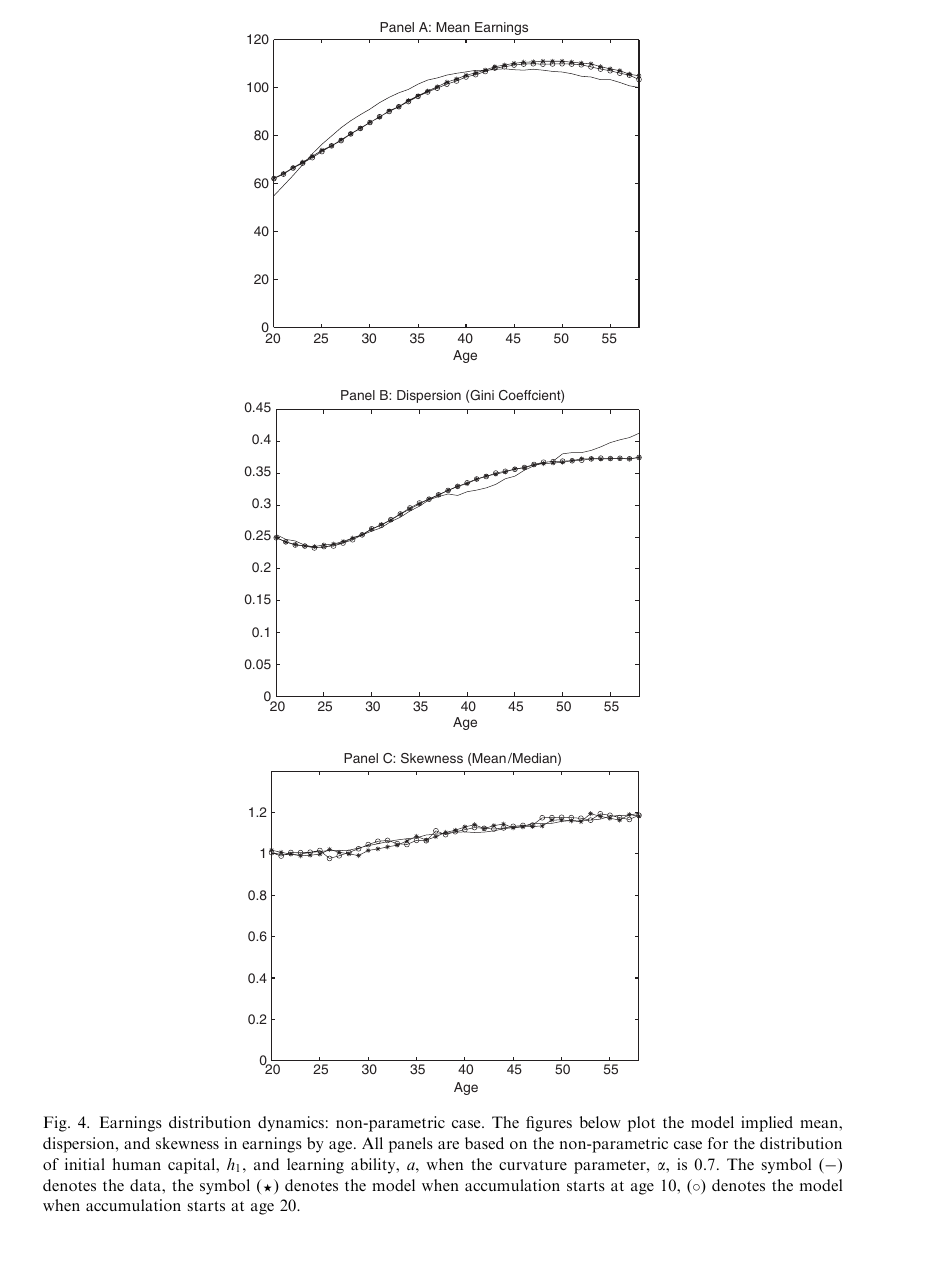
\includegraphics[height=18cm,trim=112.3 84.0 134.4 5.8,clip]{./OriginalTablesFigures/HVY2006_Figure4.png} & \includegraphics[height=18cm,trim=12.0 65.3 23.0 50.4,clip]{../SavedOutput/Graphs/HVY2006_Fig4_nonparametric.png}
\end{tabular}
\end{center}
\caption{Figure 4 of HVY2006: earnings distribution dynamics, non-parametric case, $\alpha=0.7$. Left: original from paper, where the line ($-$) is the data, ($\star$) the model with accumulation from age 10 and ($\circ$) from age 20. Right: replication.}
\label{fig:HVY2006_Fig4}
\end{figure}

\begin{figure}[htp]
\begin{center}
\begin{tabular}{cc}
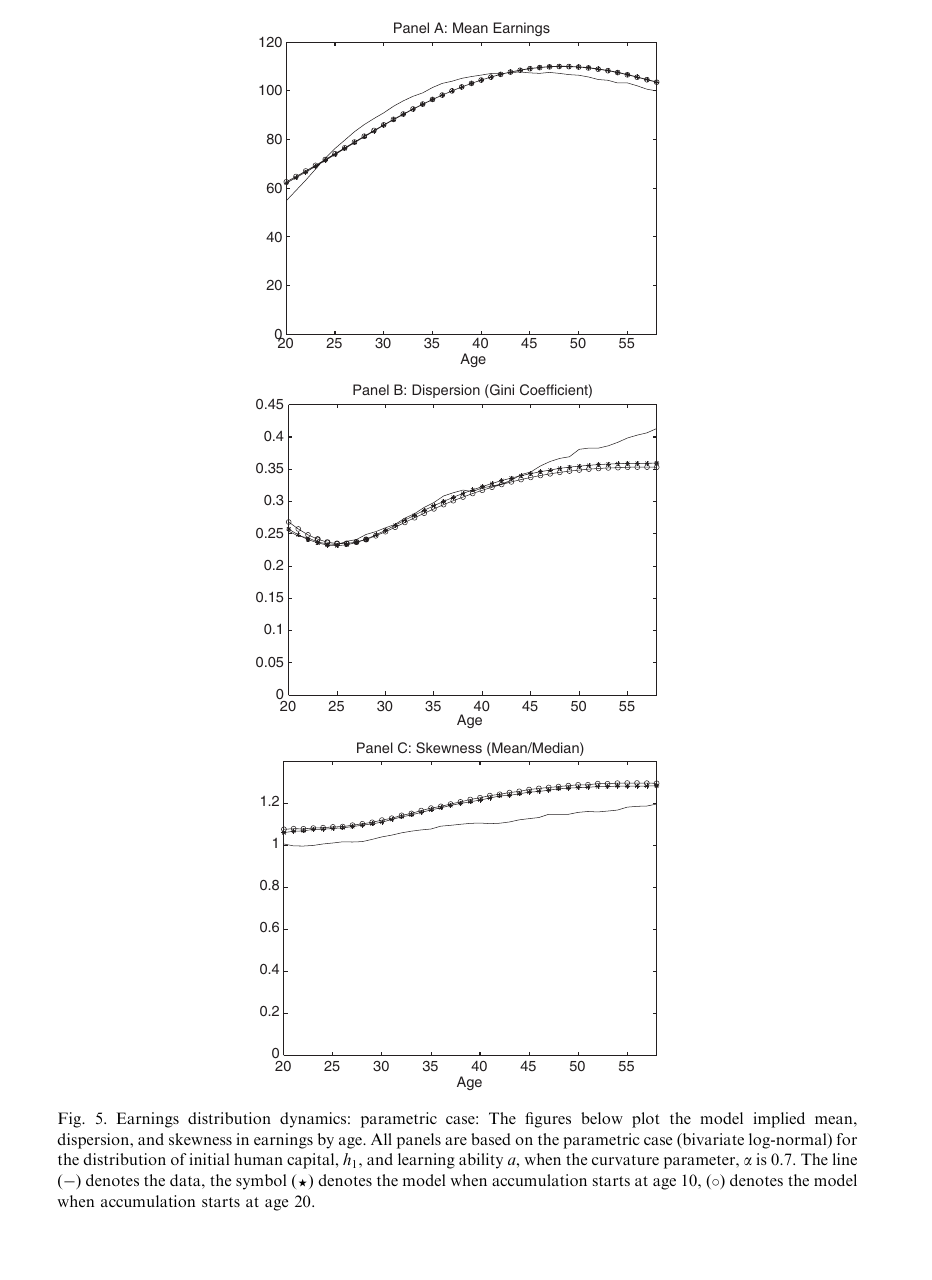
\includegraphics[height=18cm,trim=118.1 86.4 125.8 5.8,clip]{./OriginalTablesFigures/HVY2006_Figure5.png} & \includegraphics[height=18cm,trim=12.0 65.3 23.0 50.4,clip]{../SavedOutput/Graphs/HVY2006_Fig5_parametric.png}
\end{tabular}
\end{center}
\caption{Figure 5 of HVY2006: earnings distribution dynamics, parametric case, $\alpha=0.7$. Left: original from paper, where the line ($-$) is the data, ($\star$) the model with accumulation from age 10 and ($\circ$) from age 20. Right: replication.}
\label{fig:HVY2006_Fig5}
\end{figure}

\begin{figure}[htp]
\begin{center}
\begin{tabular}{cc}
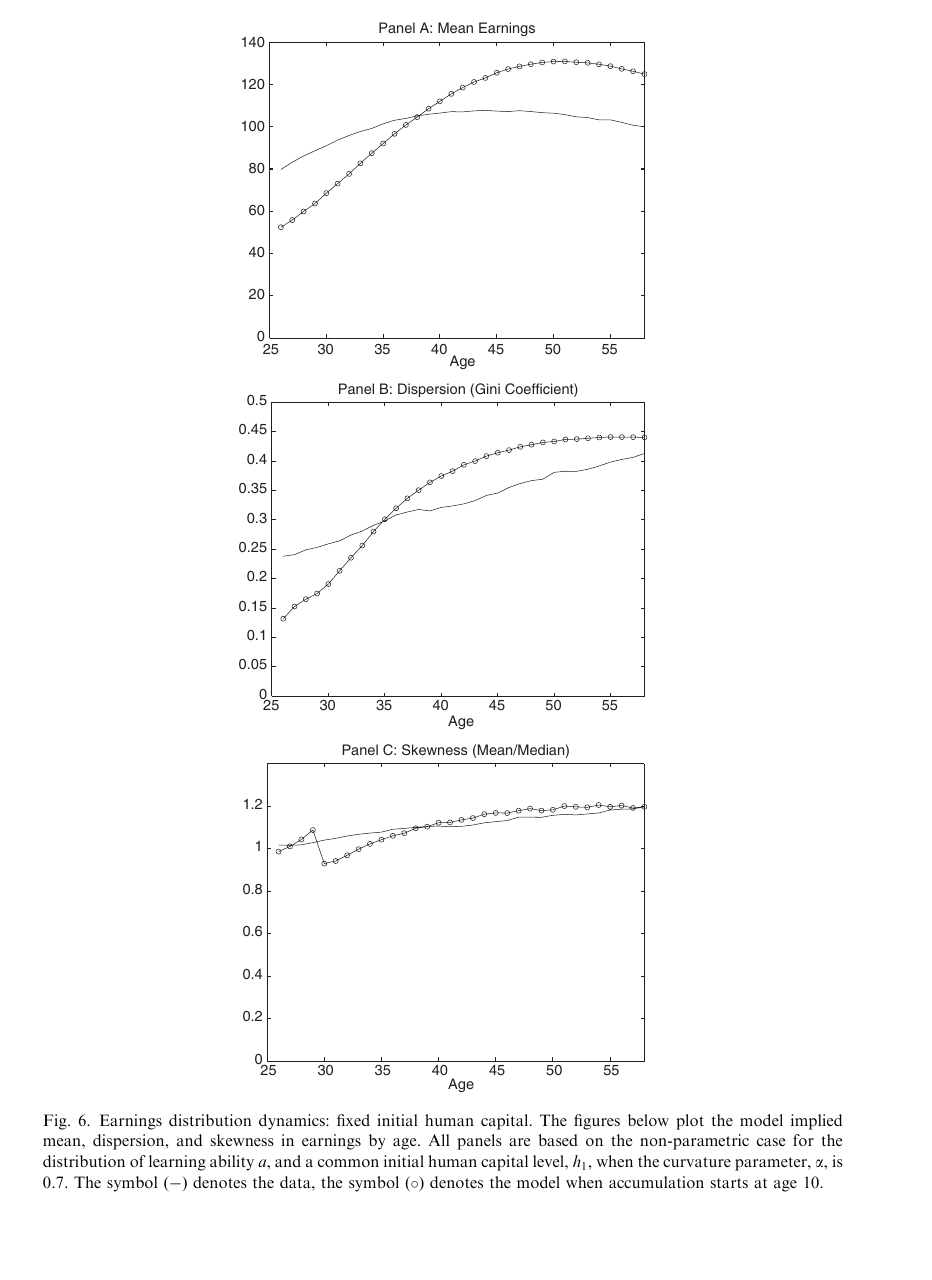
\includegraphics[height=18cm,trim=109.9 85.4 131.5 5.8,clip]{./OriginalTablesFigures/HVY2006_Figure6.png} & \includegraphics[height=18cm,trim=15.4 65.3 23.0 50.4,clip]{../SavedOutput/Graphs/HVY2006_Fig6.png}
\end{tabular}
\end{center}
\caption{Figure 6 of HVY2006: earnings distribution dynamics with a common initial human capital, non-parametric ability, $\alpha=0.7$, accumulation from age 10. Left: original from paper (which plots from age 25), where the line ($-$) is the data and ($\circ$) the model. Right: replication (from age 20).}
\label{fig:HVY2006_Fig6}
\end{figure}

\begin{figure}[htp]
\begin{center}
\includegraphics[width=120mm]{../SavedOutput/Graphs/HVY2006_Prop1.png}
\end{center}
\caption{Proposition 1(iii) of HVY2006: Gini coefficient of earnings by age in the data, the baseline model ($\alpha=0.7$, from age 20), and the same model when every agent has the mean ability. Not in HVY2006.}
\label{fig:HVY2006_Prop1}
\end{figure}


\end{document}
